
\qrchapter{https://forgottenpillar.com/rsc/en-fp-chapter23}{Ukengeufu mkuu utakuja kutimizwa hivi karibuni} \label{chap:apostasy}

Mnamo 1903, wakati The Living Temple lilipochapishwa na kuanzisha mabishano juu ya \emcap{Umbile la Mungu}, Dada White alikuwa akitii kwa uaminifu amri ya Kamanda Mkuu. Aliitwa kwa maneno “\textit{Kutana nayo!}” Alikumbana na utata huu kwa kuandika barua nyingi kwa watu wengi waliokuwa katika utumishi maeneo pote. Katika barua hizi, tunafuatilia ufahamu wa kinabii wa mustakabali wa Kanisa la Waadventista Wasabato.

Mfano mmoja ni mawasiliano kati ya Dada White na mwanawe William White. Mnamo Novemba 26, 1905, kulikuwa na Kongamano kubwa la Afya katika College View Nebraska, ambapo wafanyakazi wengi wa kimisionari wa matibabu walikutana pamoja. William White alikuwepo na alikuwa na muda mfupi, hotuba ya watu wote ya dakika 30. Baadaye, aliandika barua kwa mama yake kuhusu maoni yake kutoka katika mkutano huo. Hapa kuna sehemu ya barua hiyo:

\others{College View, Ne. – Jumanne, Novemba 28, 1905; Mwandishi: William C. White} \\
\others{Novemba 28, 1905.} \\
\others{Bi. E. G. White, Sanitarium, Cala.}

\othersnogap{...Sabato asubuhi nilipata nafasi ya kuzungumza kama dakika thelathini. Katika maelezo yangu nilirejelea kwa historia ya kanisa la Kikristo. Walianza na kanuni safi, lakini kupitia mashambulizi ya Shetani wakarudi nyuma na kuziacha kanuni hizo. \textbf{Nilielekeza kwamba tumaini pekee kwa kanisa la S. D. A. lilikuwa \underline{kuzingatia kanuni za kwanza}}. \textbf{Mimi basi narejelea mpangilio ambao adui anashambulia kazi yetu. Juhudi zake za kwanza zilikuwa kuharibu muungano na kuanzisha utengano. Kazi yake iliyofuata ilikuwa kudhoofisha heshima yetu kwa ajili ya Sabato, kisha kudhoofisha imani yetu katika huduma ya Patakatifu, kisha \underline{kuvunja imani yetu katika Roho wa Unabii}, kisha \underline{kuchanganya dhana yetu kuhusu Mungu wa kibinafsi}}.}[Letter from W. C. White to E. G. White, November 28, 1905.][http://ellenwhite.org/content/correspondence/incoming/43292pdf]

\begin{figure}
    \centering
    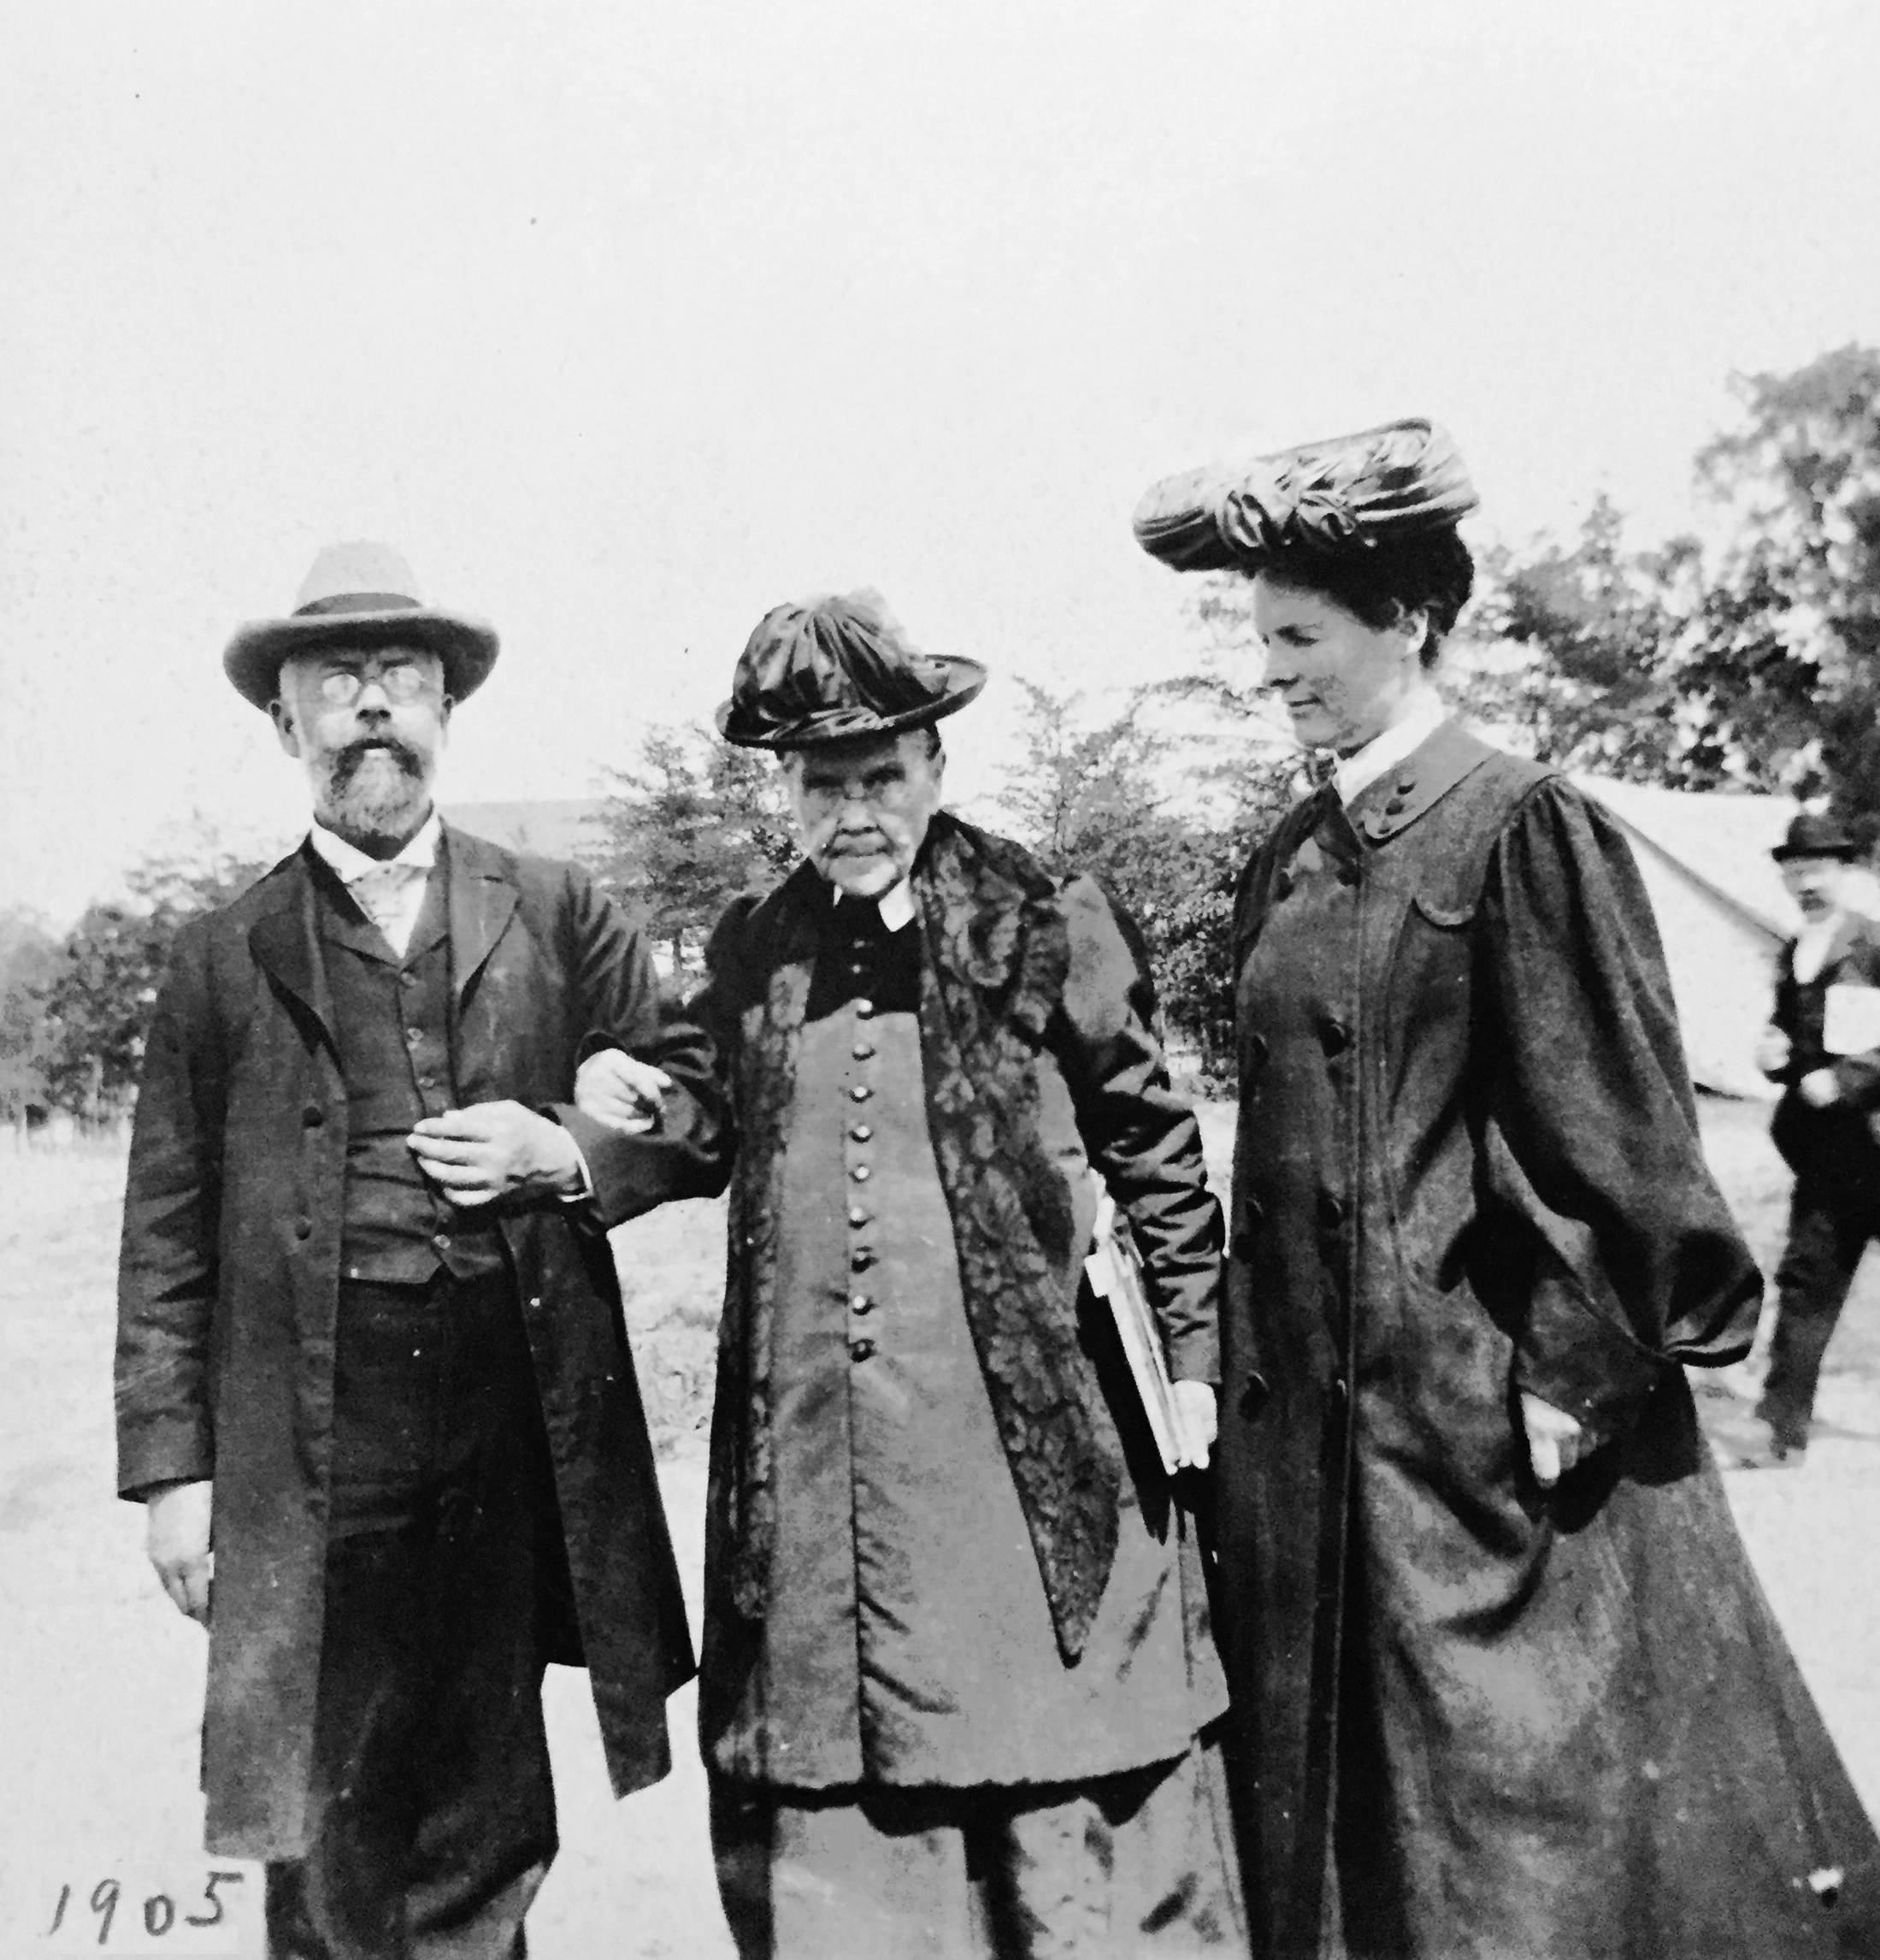
\includegraphics[width=1\linewidth]{images/william-ellen-white-1905.jpg}
    \caption*{William C. White na Ellen G. White, 1905}
    \label{fig:w-e-white}
\end{figure}

Kulingana na William White, tumaini letu pekee kama Waadventista Wasabato ni kuzingatia kanuni za kwanza. Kanuni hizi, kama tunavyojua, ni \emcap{Kanuni za Msingi}. Kisha, alitaja kwa mpangilio ambao adui anashambulia kazi yetu. Shambulio linaanza na mifarakano yetu, basi inalenga kudhoofisha heshima yetu kwa Sabato na huduma ya Patakatifu, inalenga imani yetu katika Roho ya Unabii, na hatimaye inalenga kuchanganya dhana zetu kuhusu Mungu wa kibinafsi.

Jibu la Dada White kwa William White ni la asili ya kushangaza. Anatudokezea kuwa ukengeufu mkuu utakuja kutimizwa hivi karibuni, na kwamba tumaini letu ni kuzingatia kanuni za kwanza za imani yetu—\emcap{Kanuni za Msingi}.

\egw{Elmshaven, St. Helena, California} \\
\egw{Desemba 4, 1905} \\
\egw{W. C. White} \\
\egw{Mwanangu mpendwa - }

\egw{...}

\egw{...}

\egw{“\textbf{Jambo moja ambalo ni hakika litatimizwa hivi karibuni—\underline{uasi mkubwa}, unaoendelea na kuongezeka na kuzidi kuwa na nguvu na \underline{itaendelea} kufanya hivyo mpaka Bwana atakaposhuka kutoka mbinguni kwa sauti kuu. \underline{Tunapaswa kushika kwa nguvu kanuni za kwanza za imani yetu ya kimadhehebu} na kwenda mbele kutoka nguvu hadi imani iliyoongezeka. \underline{Milele} tunapaswa kuhifadhi imani ambayo imethibitishwa na Roho Mtakatifu wa Mungu tangu matukio ya awali ya uzoefu wetu hadi wakati huu.} Sasa tunahitaji upana mkubwa zaidi na kina zaidi, imani yenye bidii zaidi, isiyoyumba-yumba katika mwongozo wa Roho Mtakatifu. \textbf{Ikiwa tulihitaji dhihirisho la uthibitisho wa uwezo wa Roho Mtakatifu kuthibitisha ukweli \underline{hapo mwanzo}, baada ya kupita kwa wakati, \underline{tunahitaji leo ushahidi wote katika uthibitisho wa ukweli}, wakati nafsi wanajitenga na imani na kutii roho zidanganyazo na mafundisho ya mashetani.} Ni lazima kusiwe na kudhoofika kwa roho sasa. Ikiwa kulikuwa na kipindi cha wakati tulipohitaji nguvu za Roho Mtakatifu katika mazungumzo yetu, katika maombi yetu, katika kila tendo lililopendekezwa, ni sasa. \textbf{Hatupaswi kuacha uzoefu wa kwanza, lakini wakati tunavumilia \underline{ujumbe huo} kwa watu, \underline{ujumbe huu unapaswa kuimarishwa na kupanuliwa}}. \textbf{Tunapaswa kuona na kutambua umuhimu wa ujumbe unaohakikishwa na asili yake ya kiungu}. Tunapaswa kufuata ili kumjua Bwana, ili tujue kwamba kutoka kwake kumetayarishwa kama vile asubuhi. Nafsi zetu zinahitaji kuhuishwa kutoka kwa Chanzo cha nguvu zote. \textbf{Tunaweza kuimarishwa na kuthibitishwa katika uzoefu uliopita \underline{ambao unatushikilia kwa mambo muhimu ya ukweli ambayo yametufanya tulivyo—Waadventista Wasabato}.}”}[Lt326-1905.2; 1905][https://egwwritings.org/read?panels=p7678.8]

\egwnogap{\textbf{Miaka hamsini iliyopita haijafifisha yodi moja au kanuni ya imani yetu kama tulivyopokea ushahidi mkubwa na wa ajabu ambao ulifanywa kuwa hakika kwetu mnamo 1844, baada ya kupita kwa wakati.} Roho zinazodhoofika zinapaswa kuthibitishwa na kuhuishwa kulingana na Neno Lake. Na wengi wa wahudumu wa injili na waganga wa Bwana walio na roho zinazodhoofika zitahuishwa kulingana na Neno. \textbf{\underline{Hakuna neno linalobadilishwa au kukataliwa}.} \textbf{Yale ambayo Roho Mtakatifu alishuhudia kuwa ni kweli baada ya kupita kwa wakati, katika kukatishwa tamaa kuu, ndio \underline{msingi thabiti wa ukweli}. Nguzo za ukweli zilifunuliwa, na tulikubali \underline{kanuni za msingi} ambazo zimetufanya tulivyo—Waadventista Wasabato, wazishikao amri za Mungu na kuwa na imani ya Yesu.}}[Lt326-1905.3; 1905][https://egwwritings.org/read?panels=p7678.9]

Barua hii inashangaza kwa sababu ni jibu la mpangilio wa jinsi adui anavyoshambulia kazi yetu. Dada White anafahamu vyema mashambulizi haya na aliwasilisha tatizo hili kwa nuru yake sahihi, pia akituonyesha kile tutakachofanya ili kuzuia mashambulizi ya Shetani juu yetu. Adui anataka \others{kuchanganya dhana yetu kuhusu Mungu wa kibinafsi}. Hii ni hatua ya ukengeufu mkuu ambao \egwinline{utatimizwa hivi karibuni}, na umekuwa \egwinline{ukiendelea na kuongezeka na kuongezeka nguvu zaidi na itaendelea kufanya hivyo mpaka Bwana atakaposhuka kutoka mbinguni pamoja na mwaliko}. Huu ndio ukengeufu tunaoupata leo. Nini matumaini yetu dhidi ya udanganyifu huu na uasi mkuu? \egwinline{\textbf{\underline{Tunapaswa kushikilia kwa dhati kanuni za kwanza za imani yetu ya kimadhehebu} na kwenda mbele kutoka kwa nguvu hadi imani iliyoongezeka. \underline{Daima} tunapaswa kutunza imani yetu ambayo imethibitishwa na Roho Mtakatifu wa Mungu kutokana na matukio ya awali ya uzoefu wetu mpaka wakati huu.}} \egwinline{...\textbf{\underline{ujumbe huu unapaswa kuimarishwa na kukuzwa}}...} \egwinline{...\textbf{\underline{tunahitaji leo ushahidi wote katika uthibitisho wa ukweli}}...} \egwinline{\textbf{Tunaweza kuimarishwa na kuthibitishwa katika uzoefu uliopita ambao unatushikilia kwa muhimu mambo ya ukweli ambayo yametufanya tuwe hivi tulivyo—Waadventista Wasabato}}. Haya mambo muhimu ya ukweli, ambayo yametufanya sisi Waadventista Wasabato, ndiyo \emcap{Kanuni za Kimsingi}, zilizozaliwa mwanzoni mwa kazi yetu. Mnamo 1905, aliandika, \egwinline{\textbf{Miaka hamsini iliyopita haijafifisha yodi moja au kanuni ya imani yetu kama tulivyopokea ushahidi mkubwa na wa ajabu ambao ulifanywa kuwa hakika kwetu mnamo 1844, baada ya kupita kwa wakati.}} \egwinline{\textbf{\underline{Hakuna neno linalobadilishwa au kukataliwa}.} \textbf{Yale ambayo Roho Mtakatifu alishuhudia kuwa ni kweli baada ya kupita kwa wakati, katika kukatishwa tamaa kuu, ndio \underline{msingi thabiti wa ukweli}. Nguzo za ukweli zilifunuliwa, na tulikubali \underline{kanuni za msingi} ambazo zimetufanya tulivyo—Waadventista Wasabato, wazishikao amri za Mungu na kuwa na imani ya Yesu.}}

Mungu anatuita kuwa imara katika \emcap{Kanuni za Kimsingi}, hasa juu ya \others{dhana kuhusu Mungu binafsi}. Hili ni jambo la kwanza la \emcap{Kanuni za Kimsingi}.

Dada White alitabiri kwamba ukengeufu mkubwa unaendelea katika kanisa letu kuhusu ufahamu wa \emcap{Umbile la Mungu}. Ufahamu wa kweli wa \emcap{Umbile la Mungu} umewasilishwa katika \emcap{Kanuni za Kimsingi}. Alituonya waziwazi kuhusu shambulio la Shetani dhidi ya kanuni hizi. Anatuita \egw{\textbf{kushikilia sana kanuni za kwanza za imani yetu ya kimadhehebu} na kwenda mbele kutoka nguvu hadi imani iliyoongezeka}.

\egw{\textbf{“Baada ya muda kupita, Mungu aliwakabidhi wafuasi Wake waaminifu vitu vya thamani \underline{kanuni za ukweli wa sasa}. Kanuni hizi hazikutolewa kwa wale ambao hawakuwa na sehemu katika utoaji wa ujumbe wa malaika wa kwanza na wa pili. Walipewa kwa wafanyakazi ambao walikuwa na sehemu katika kazi hiyo tangu mwanzo}.”}[Ms129-1905.5; 1905][https://egwwritings.org/read?panels=p9797.12]

\egwnogap{\textbf{Wale ambao walipitia uzoefu huu wanapaswa kuwa \underline{thabiti kama mwamba kwa kanuni} ambazo zimetufanya kuwa Waadventista Wasabato}. Wanapaswa kuwa wafanyakazi pamoja na Mungu, akifunga ushuhuda na kutia muhuri sheria kati ya wanafunzi wake. Wale waliochukua sehemu katika kusimamisha kazi yetu juu ya msingi wa kweli ya Biblia; \textbf{wale wanaojua viashiria njia ambavyo vimeonyesha njia sahihi} wanapaswa kuzingatiwa kama wafanyikazi wa thamani ya juu. Wanaweza kusema kutokana na uzoefu wa kibinafsi, kuhusu kweli walizokabidhiwa wao. Watu hawa hawapaswi kuruhusu imani yao ibadilishwe na kuwa ukafiri; hawatakiwi kuruhusu bendera ya malaika wa tatu kuchukuliwa kutoka mikononi mwao. Wanapaswa kushikilia mwanzo wa imani yao imara hadi mwisho. \textbf{\underline{Bwana ametangaza kwamba historia iliyopita itarudiwa tunapoingia kwenye kazi ya utimisho}. Kila ukweli alionao iliyotolewa kwa ajili ya siku hizi za mwisho itatangazwa kwa ulimwengu. \underline{Kila nguzo} imara aliyotengeneza \underline{itaimarishwa}. Hatuwezi sasa kuondoa kwa msingi ambao Mungu ameanzisha. Hatuwezi sasa kuingia katika shirika lolote jipya; kwa maana hii ni kuasi kutoka kwa ukweli}.}[Ms129-1905.6; 1905][https://egwwritings.org/read?panels=p9797.13]

Kuondoka kwenye msingi ambao Mungu ameweka kunamaanisha kuingia katika shirika jipya; huu ni ukengeufu kutoka kwa ukweli. Kulinganisha \emcap{Kanuni za Kimsingi} za zamani na Imani za Msingi za utatu wa sasa, ni dhahiri tuko katika hali ya ukengeufu. Ellen White alitabiri kwamba ukengeufu huu utakuwa \egwinline{\textbf{ukiendelea na kuongezeka na kukua kwa nguvu zaidi na \underline{itaendelea} kufanya hivyo hadi Bwana atakaposhuka kutoka mbinguni kwa ukemi}}[Lt326-1905.2; 1905][https://egwwritings.org/read?panels=p7678.8].

% The great apostasy is soon to be realized

\begin{titledpoem}
    
    \stanza{
        In a letter penned, a crisis foretold, \\
        From Ellen White, a warning bold: \\
        "Adhere to the roots of our Adventist comprehend, \\
        For soon will come apostasy's seed."
    }

    \stanza{
        The pillars strong of our founding year, \\
        Are under siege, as Ellen feared. \\
        To "Meet it!" was her stern command, \\
        To hold the line, to firmly stand.
    }

    \stanza{
        "Keep to the principles," her urgent plea, \\
        From 1844's prophetic decree. \\
        For truth confirmed by the Spirit's flame, \\
        Shall not be denied, nor put to shame.
    }

    \stanza{
        The enemy seeks to divide and sway, \\
        To change our course, to lead astray. \\
        But steadfast hearts must ever cling \\
        To the first truths that made our spirits sing.
    }

    \stanza{
        Hold fast, she wrote, to what we know, \\
        The Fundamental Principles that show \\
        The way to live, the path to trod, \\
        Under the gaze of an unchanging God.
    }

    \stanza{
        For as the world spins toward its close, \\
        The truth of Ellen White still glows— \\
        A beacon strong against the night, \\
        Guiding the faithful in the right.
    }
    
\end{titledpoem}
